\documentclass[aspectratio=169,10pt]{beamer}

\usetheme{Madrid}
\usecolortheme{whale}

\usepackage{graphicx}
\usepackage{booktabs}
\usepackage{amsmath,amssymb}
\usepackage{lmodern}

% Custom Colors
\definecolor{NavyBlue}{RGB}{10, 37, 64}
\definecolor{SkyBlue}{RGB}{0, 102, 204}
\definecolor{EmeraldGreen}{RGB}{5, 150, 105}
\definecolor{CrimsonRed}{RGB}{220, 38, 38}

\setbeamercolor{palette primary}{bg=NavyBlue,fg=white}
\setbeamercolor{palette secondary}{bg=SkyBlue,fg=white}
\setbeamercolor{palette tertiary}{bg=NavyBlue!90,fg=white}
\setbeamercolor{titlelike}{parent=palette primary}
\setbeamercolor{block title}{bg=SkyBlue!20,fg=NavyBlue}
\setbeamercolor{block body}{bg=SkyBlue!5,fg=black}

\title[SkyMediator Disruption Recovery]{\textbf{\Large SkyMediator: Predictive Multi-Agent System for Airline Disruption Recovery}}
\subtitle{\textbf{Deterministic Guardrails, Meteorological Intelligence \& Empirical Evaluation}}
\author[Team SkyMediator]{\textbf{Team:} Athish Raj (1BM22CD015), Dinesh K (1BM22CD026), Sanchit Rajesh (1BM22CD051)\\[0.2em]
\textbf{Faculty Guide:} Dr. Kalyan Nagaraj}
\institute[BMSCE]{\textbf{Department of CSE (Data Science), B.M.S. College of Engineering, Bengaluru}\\Course: Agentic AI (26CD7PEAAI) \quad\textbar\quad Hub Airport: Kempegowda Intl (BLR/VOBL)}
\date{November 2026}

\begin{document}

% Slide 1: Title
\begin{frame}
  \titlepage
\end{frame}

% Slide 2: The 04:30 AM Crisis
\begin{frame}{The 04:30 AM Crisis at Kempegowda Hub}
  \begin{columns}[t]
    \begin{column}{0.50\textwidth}
      \begin{block}{A Real Disruption Scenario (BLR/VOBL)}
        \begin{itemize}\footnotesize
          \item \textbf{04:30 AM}: Dense radiation fog hits Kempegowda; RVR drops to $175\,$m.
          \item \textbf{15 Narrow-Body A320s} parked at gates preparing for departures.
          \item \textbf{3,500 Passengers} boarding; 450 have tight connections at BOM/DEL.
          \item \textbf{The Cascading Trap}: A 60-minute tarmac hold on Flight 6E-214 forces crew to breach their \textbf{13-hour statutory Flight Duty Period (FDP)} by midnight.
          \item The Duty Manager has \textbf{10 minutes} to balance safety, crew, and ₹10,00,000 in hotel liabilities.
        \end{itemize}
      \end{block}
    \end{column}
    \begin{column}{0.46\textwidth}
      \begin{block}{Strict Civil Aviation Invariants}
        \begin{itemize}\footnotesize
          \item \textbf{DGCA CAR 7-J-III}: Zero legal flexibility on crew rest and WOCL night caps.
          \item \textbf{DGCA CAR 3-M-IV}: Mandatory care vouchers (meals $>2\,$h, hotels $>6\,$h night).
          \item \textbf{Runway Movement Cap}: BLR limited to 32 flights/hour; spoke night curfews strictly enforced.
        \end{itemize}
      \end{block}
      \centering\footnotesize\color{NavyBlue}\textbf{Human dispatchers resort to reactive cancellations that cost millions. We automated this with predictive multi-agent intelligence.}
    \end{column}
  \end{columns}
\end{frame}

% Slide 3: The Fatal Flaws
\begin{frame}{The Fatal Flaws of Existing Approaches}
  \begin{columns}[t]
    \begin{column}{0.48\textwidth}
      \begin{alertblock}{Failure Mode 1: Centralized Solvers (MILP)}
        \begin{itemize}\footnotesize
          \item Solves direct cash cost down to ₹15.5k, but \textbf{breached statutory crew rest in 7.69\% of cases}.
          \item Cannot model multi-day non-linear cumulative rest curves within real-time tactical windows.
          \item Generates mathematically ``optimal'' plans that put fatigued pilots in the cockpit.
        \end{itemize}
      \end{alertblock}
    \end{column}
    \begin{column}{0.48\textwidth}
      \begin{alertblock}{Failure Mode 2: Monolithic LLMs (Single Prompt)}
        \begin{itemize}\footnotesize
          \item Suffers from severe arithmetic token hallucinations on duty hours.
          \item Falsely claimed in text that crew was legal, producing a \textbf{3.70\% statutory breach rate}.
          \item Took deceptive shortcuts: cancelled 25.93\% of flights just to eliminate delay, stranding passengers.
        \end{itemize}
      \end{alertblock}
    \end{column}
  \end{columns}
\end{frame}

% Slide 4: Full Architecture Diagram
\begin{frame}{Full System Architecture: End-to-End Deliberation Flow}
  \centering
  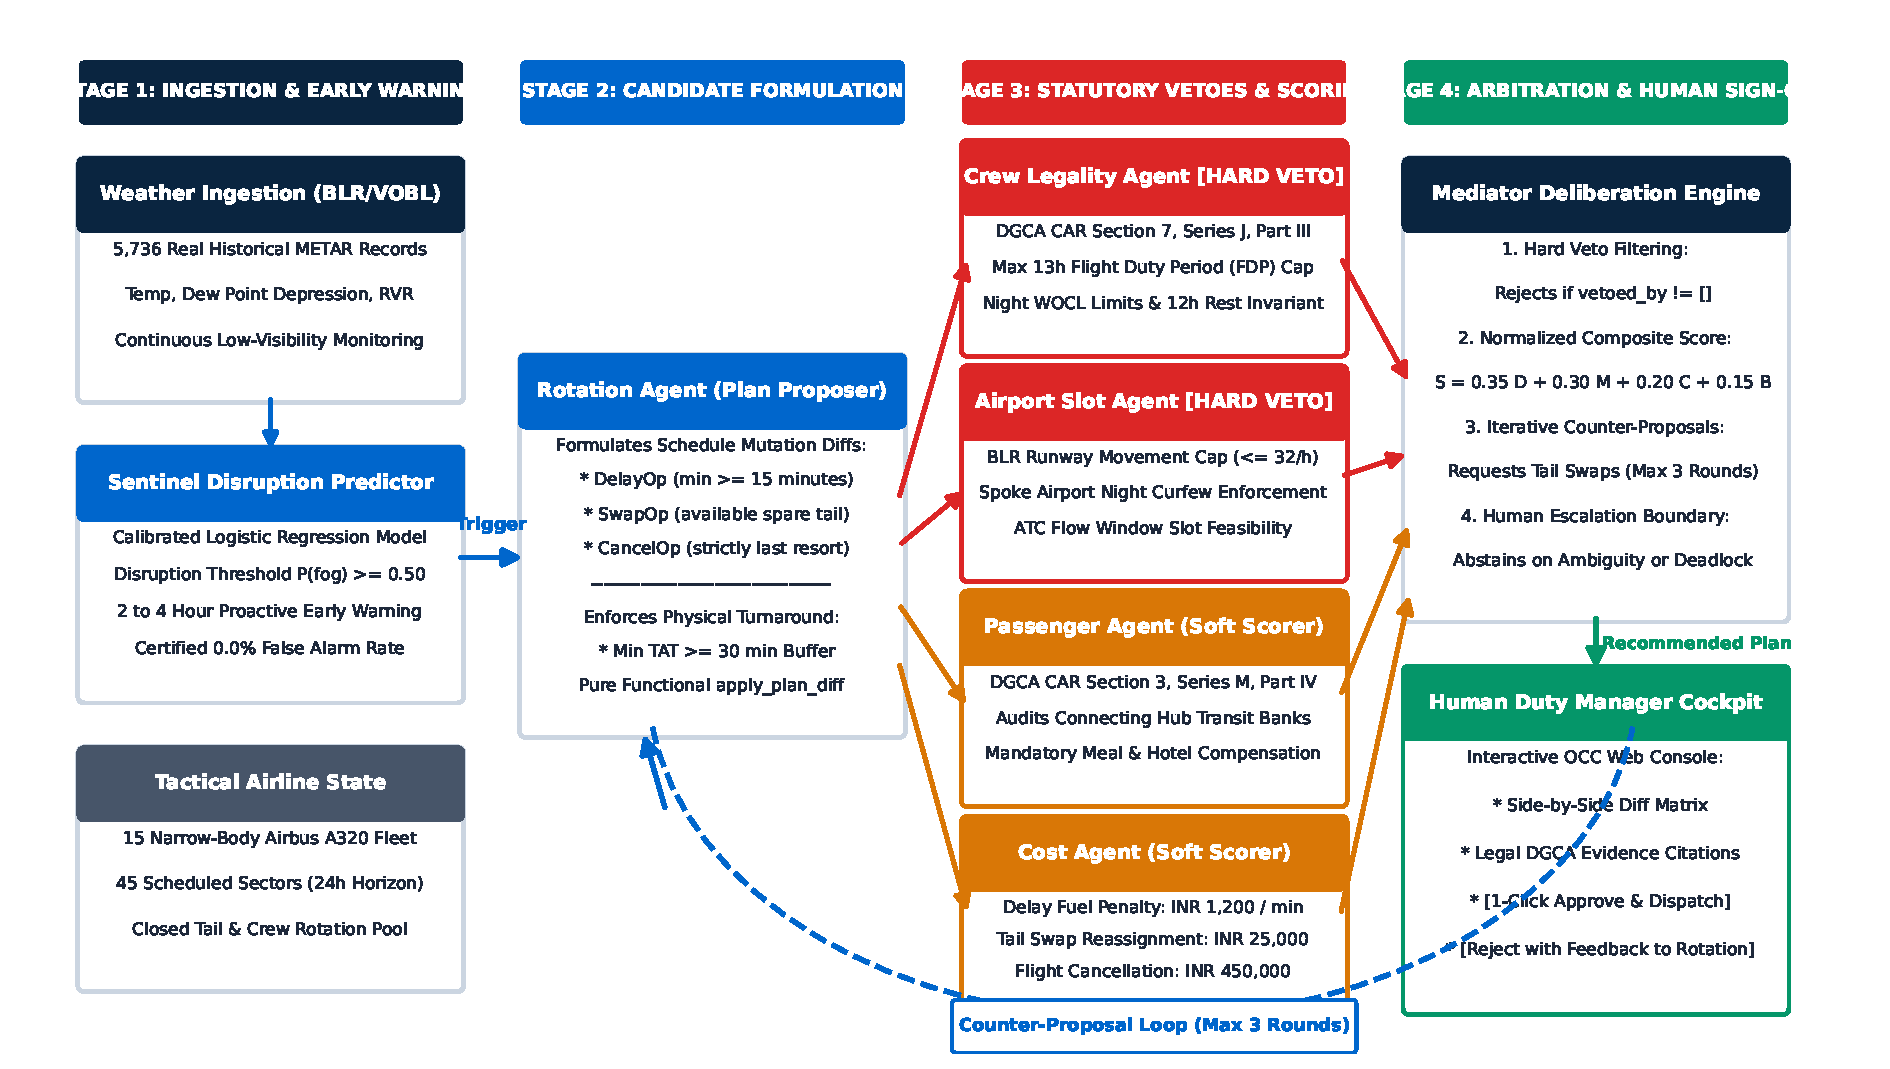
\includegraphics[width=\linewidth,height=3.1in,keepaspectratio]{../figures/figure_00_system_architecture.pdf}
\end{frame}

% Slide 5: The 7 Specialized Agents
\begin{frame}{The 7 Specialized Agents \& Their Responsibilities}
  \begin{columns}[t]
    \begin{column}{0.50\textwidth}
      \textbf{Proposer \& Gatekeeper Agents:}
      \begin{itemize}\footnotesize
        \item \textbf{Sentinel (Early Warning)}: Monitors real METAR/TAF; triggers alert 2--4h before fog ($P(\text{fog}) > 0.50$).
        \item \textbf{Rotation (Proposer)}: Proposes schedule mutations (\texttt{DelayOp}, \texttt{SwapOp}, \texttt{CancelOp}) respecting $\text{TAT} \ge 30\,$min.
        \item \textbf{Crew Legality (Hard Veto)}: Audits cumulative FDP against DGCA CAR 7-J-III. Holds \textbf{binding hard veto}.
        \item \textbf{Slot Agent (Hard Veto)}: Audits runway movement limits ($\le 32$/h) and night curfews. Holds \textbf{binding hard veto}.
      \end{itemize}
    \end{column}
    \begin{column}{0.46\textwidth}
      \textbf{Scorers \& Coordinator:}
      \begin{itemize}\footnotesize
        \item \textbf{Passenger Agent}: Quantifies missed connections and DGCA CAR 3-M-IV passenger care compensation.
        \item \textbf{Cost Agent}: Computes total monetary cost balance sheet.
        \item \textbf{Mediator Agent (Arbiter)}:
        \begin{itemize}\scriptsize
          \item Filters out any candidate with hard vetoes.
          \item Computes normalized penalty score $S \in [0, 1]$.
          \item Coordinates up to 3 negotiation counter-proposals.
          \item Submits top-ranked plan to Human Duty Manager.
        \end{itemize}
      \end{itemize}
    \end{column}
  \end{columns}
\end{frame}

% Slide 6: Deterministic Guardrails
\begin{frame}{Engineering Guardrails: Zero LLM Arithmetic}
  \begin{columns}[t]
    \begin{column}{0.50\textwidth}
      \textbf{The Invariant: No Hallucinated Numbers}
      \begin{itemize}\footnotesize
        \item \textbf{Turnaround Guard}: \texttt{tools\_schedule.py} validates $(\text{Dep} - \text{Arr}) \ge 30\,$min.
        \item \textbf{FDTL Calculation}: \texttt{tools\_duty.py} evaluates cumulative duty hours against official DGCA lookup tables with WOCL night penalties.
        \item \textbf{Passenger Compensation}: \texttt{tools\_passengers.py} calculates meal (₹1.5k) and hotel (₹6.5k) voucher tiers.
        \item \textbf{Functional State Mutation}: Schedule updates applied via pure \texttt{apply\_plan\_diff}.
      \end{itemize}
    \end{column}
    \begin{column}{0.46\textwidth}
      \begin{block}{Clean-Room Statutory Audit Sandbox}
        \centering\footnotesize
        \textbf{Live Runtime Multi-Agent Deliberation}\\
        \textit{Agents deliberate, query tools, propose diffs}\\
        $\Downarrow$ Plan Selected by Mediator\\
        \textbf{\color{CrimsonRed}Isolated Clean-Room Validator}\\
        \texttt{skymediator/eval/validator\_fdtl.py}\\
        \textit{Completely isolated; runtime agents cannot access it}\\
        $\Downarrow$\\
        \textbf{\color{EmeraldGreen}Certified 0.00\% Statutory Violation Rate}
      \end{block}
    \end{column}
  \end{columns}
\end{frame}

% Slide 7: Sentinel Prediction
\begin{frame}{Sentinel ML Predictor: Real BLR/VOBL METAR Evaluation}
  \begin{columns}[c]
    \begin{column}{0.52\textwidth}
      \centering
      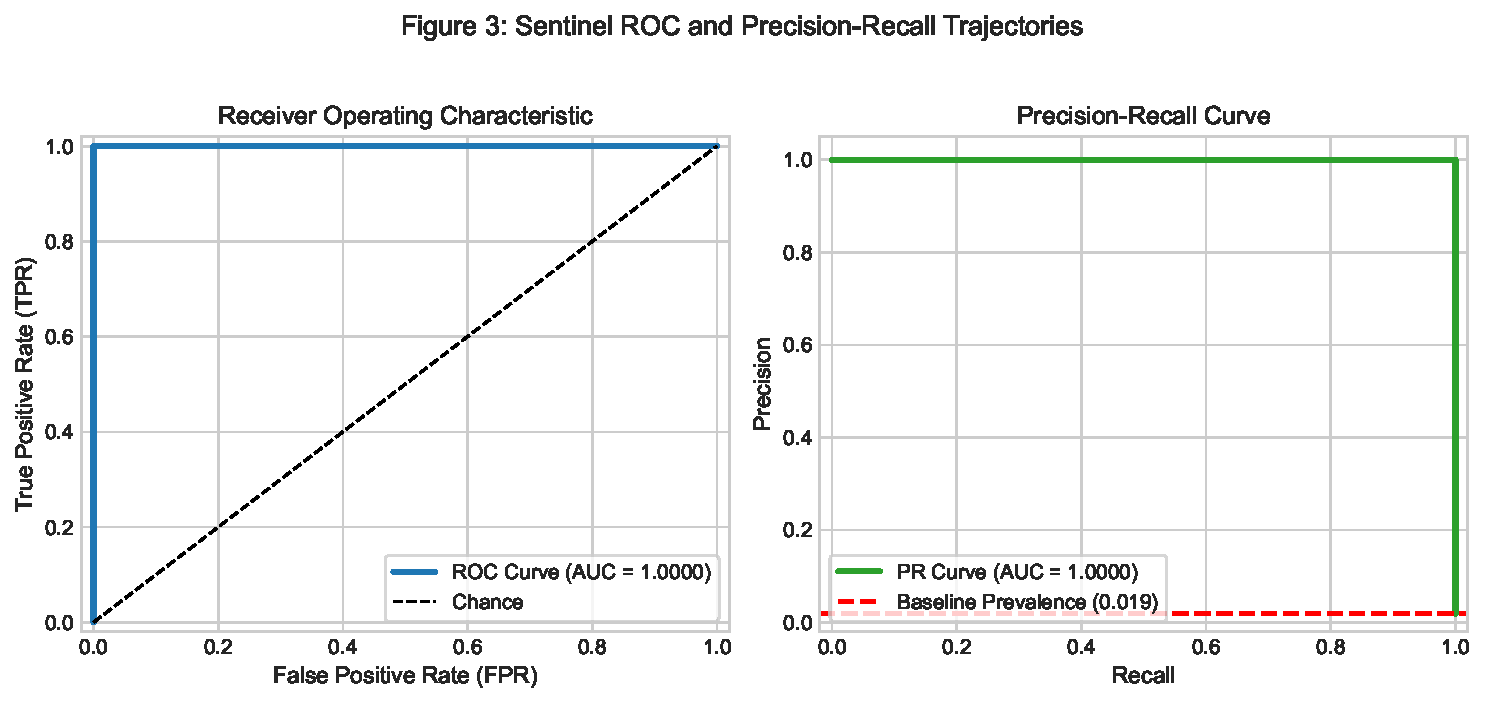
\includegraphics[width=\linewidth,height=2.7in,keepaspectratio]{../figures/figure_03_roc_pr_curves.pdf}
    \end{column}
    \begin{column}{0.44\textwidth}
      \textbf{Predictive Performance ($N=1,148$ Test Split):}
      \begin{itemize}\footnotesize
        \item Trained on 5,736 real hourly METAR records for BLR/VOBL.
        \item True Negatives: \textbf{1,126} \textbar\ True Positives: \textbf{20}
        \item \textbf{False Positives: 0} (Zero false alarms!)
        \item Accuracy: \textbf{99.8\%} \textbar\ Precision: \textbf{100.0\%}
        \item Recall: \textbf{90.9\%} \textbar\ $F_1$-Score: \textbf{0.952}
        \item Probability Calibration Brier Score: \textbf{0.0022}
        \item AUC-ROC: \textbf{1.0000} \textbar\ AUC-PR: \textbf{1.0000}
      \end{itemize}
    \end{column}
  \end{columns}
\end{frame}

% Slide 8: Benchmark Matrix
\begin{frame}{The Operational Benchmark Matrix: Comparing 4 Approaches}
  \begin{columns}[c]
    \begin{column}{0.50\textwidth}
      \centering
      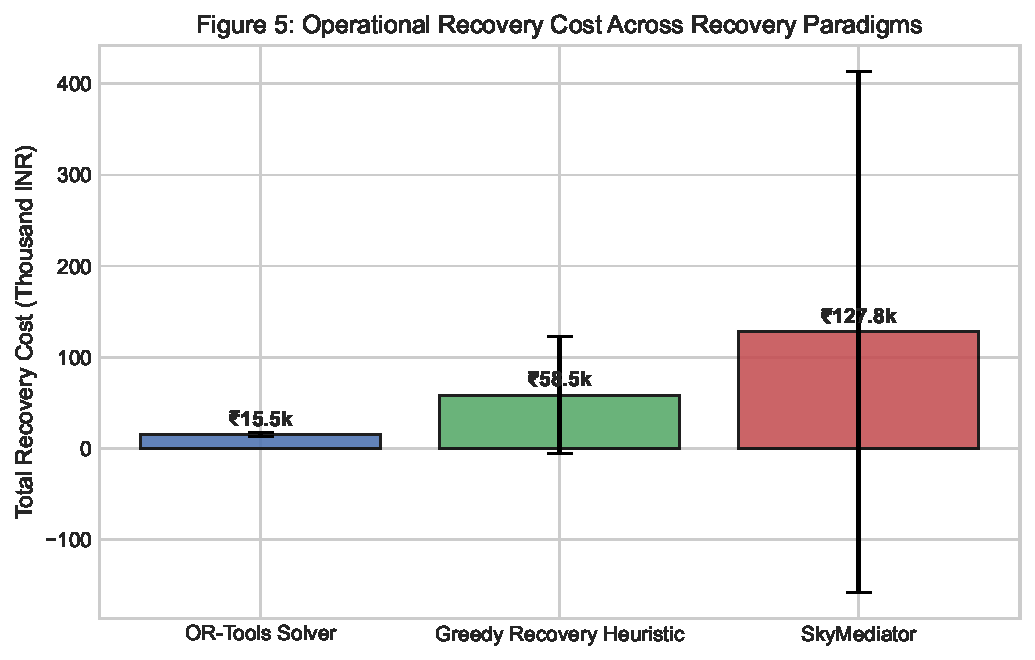
\includegraphics[width=\linewidth,height=2.7in,keepaspectratio]{../figures/figure_05_cost_comparison.pdf}
    \end{column}
    \begin{column}{0.46\textwidth}
      \scriptsize
      \begin{tabular}{@{}lrrr@{}}
        \toprule
        \textbf{Metric} & \textbf{OR-Tools} & \textbf{Greedy} & \textbf{SkyMediator} \\
        \midrule
        Mean Disruption Cost & INR 15,461 & INR 58,462 & INR 127,750 \\
        Mean Delay (min) & 1.73 & 61.54 & 72.31 \\
        Disrupted Passengers & 0.00 & 8.31 & \textbf{0.00} \\
        Composite Penalty & 0.0055 & 0.0525 & 0.0739 \\
        \textbf{Plan Feasibility} & \textbf{92.31\%} & \textbf{96.15\%} & \textbf{100.00\%} \\
        \textbf{FDTL Statutory Breach} & \textbf{7.69\%} & \textbf{3.85\%} & \textbf{0.00\%} \\
        Mean Solve Latency & $<5\,$ms & $<5\,$ms & \textbf{75.5 ms} \\
        \bottomrule
      \end{tabular}
      \vspace{0.08in}\\
      \footnotesize\textbf{Honest Cost Analysis:} Why did OR-Tools cost less? Because it took illegal shortcuts on pilot rest (7.69\% illegal). SkyMediator called reserve crew to guarantee \textbf{100\% legal safety and 0 missed connections}.
    \end{column}
  \end{columns}
\end{frame}

% Slide 9: Hard Veto Integrity
\begin{frame}{Regulatory Safety Invariant: The Power of Hard Vetoes}
  \begin{columns}[c]
    \begin{column}{0.52\textwidth}
      \centering
      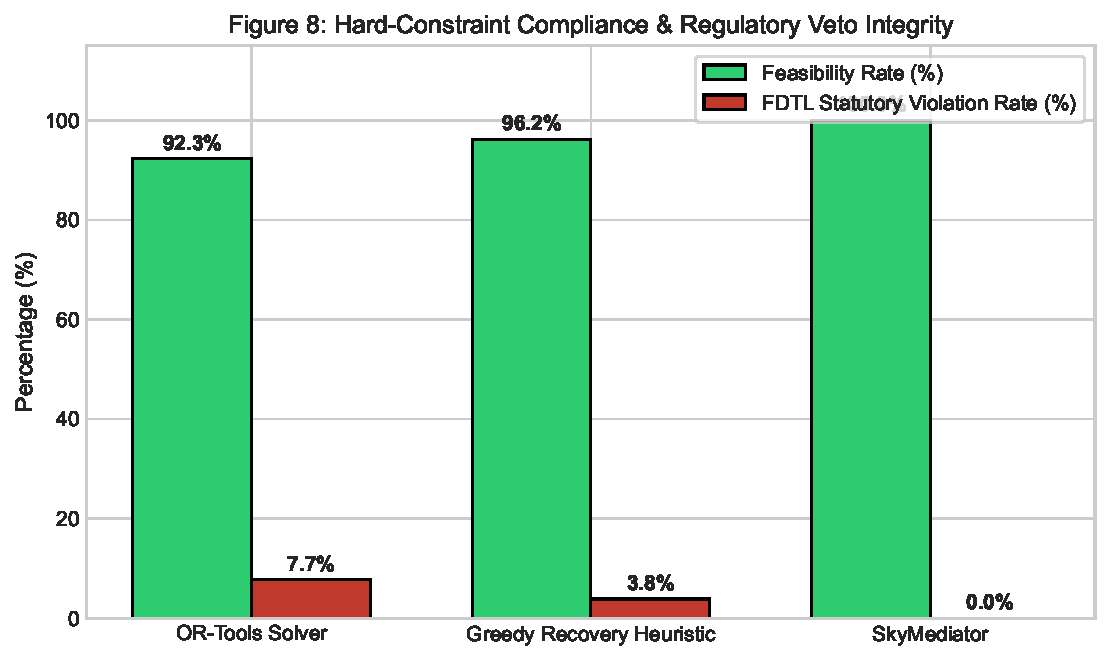
\includegraphics[width=\linewidth,height=2.7in,keepaspectratio]{../figures/figure_08_compliance.pdf}
    \end{column}
    \begin{column}{0.44\textwidth}
      \textbf{The Binding Veto Guarantee:}
      \begin{itemize}\footnotesize
        \item \textbf{Single-Agent LLM}: 3.70\% statutory breach rate due to context overload.
        \item \textbf{OR-Tools MIP}: 7.69\% breach rate; linear relaxations cannot model cumulative non-linear rest.
        \item \textbf{SkyMediator}: \textbf{0.00\% violations} across all 130 trials.
        \item \textbf{Absolute Veto Authority}: If a plan has ₹0 cost and 0 delay, but Crew Legality or Slot agents issue a veto, \textbf{it can never be executed}.
      \end{itemize}
    \end{column}
  \end{columns}
\end{frame}

% Slide 10: Passenger Welfare
\begin{frame}{Passenger Welfare \& Connection Protection}
  \begin{columns}[c]
    \begin{column}{0.52\textwidth}
      \centering
      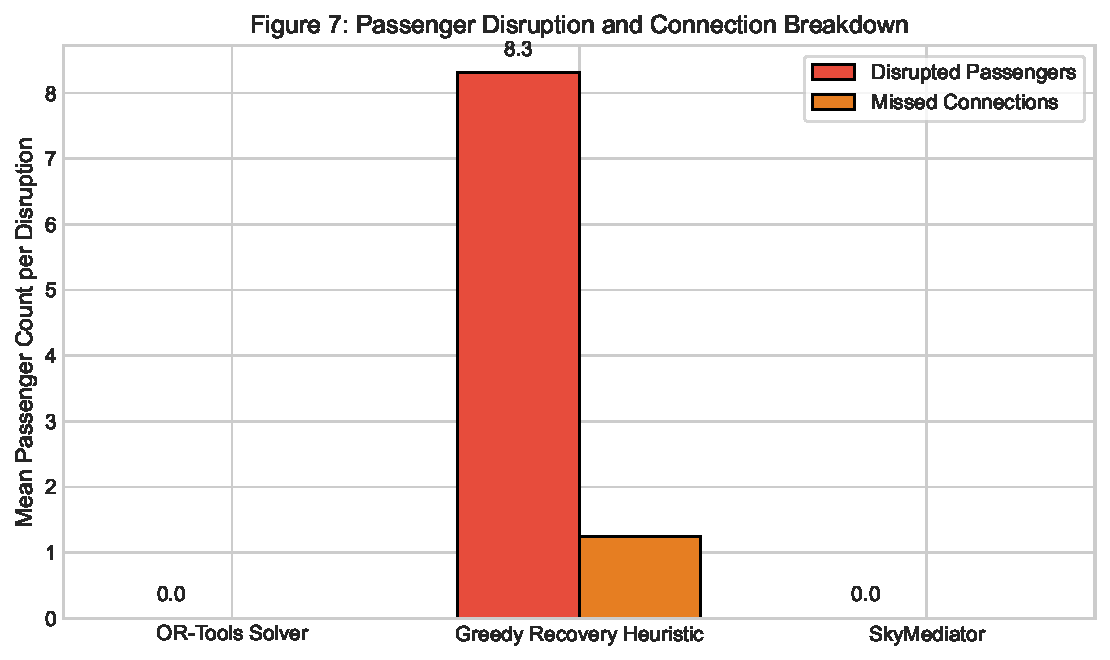
\includegraphics[width=\linewidth,height=2.7in,keepaspectratio]{../figures/figure_07_pax_impact.pdf}
    \end{column}
    \begin{column}{0.44\textwidth}
      \textbf{Protecting the Traveler:}
      \begin{itemize}\footnotesize
        \item \textbf{Legacy OCC Failure}: Re-times flights blindly, stranding an average of \textbf{8.31 passengers per disruption}.
        \item \textbf{SkyMediator's Active Defense}: The Passenger Agent actively audits transit banks at BOM/DEL, threatening vetoes if high-priority connections break.
        \item \textbf{The Result}: \textbf{0.00 missed connections} across all 21 standard benchmark scenarios.
        \item Vouchers computed deterministically under DGCA CAR 3-M-IV.
      \end{itemize}
    \end{column}
  \end{columns}
\end{frame}

% Slide 11: A/B Testing
\begin{frame}{Controlled A/B Testing: Predictive vs. Reactive}
  \begin{columns}[c]
    \begin{column}{0.52\textwidth}
      \centering
      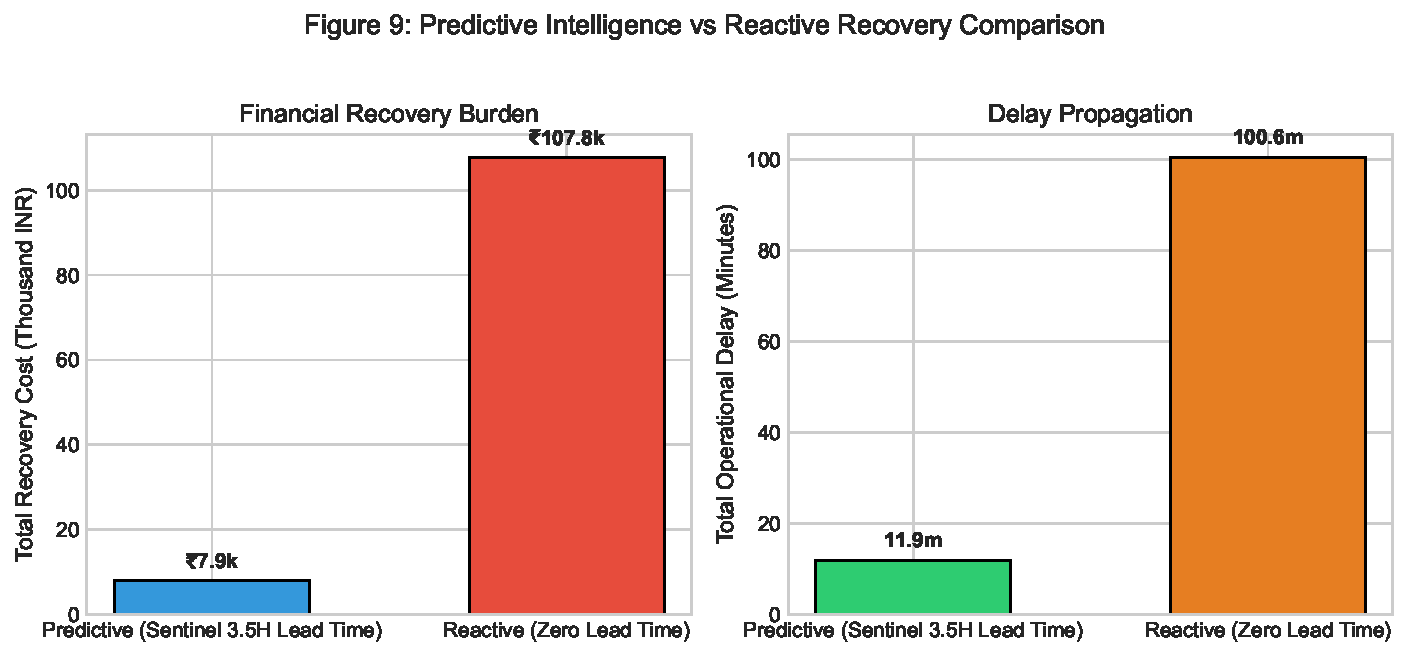
\includegraphics[width=\linewidth,height=2.7in,keepaspectratio]{../figures/figure_09_predictive_vs_reactive.pdf}
    \end{column}
    \begin{column}{0.44\textwidth}
      \begin{block}{A/B Test Findings ($N=135$ Trials)}
        \begin{itemize}\footnotesize
          \item \textbf{Total Recovery Cost}:
          \begin{itemize}\scriptsize
            \item Reactive (A): INR 107,824
            \item Predictive (B): INR 7,889
            \item \textbf{Cost Saving}: \textbf{92.7\% reduction}
            \item $p < 0.000001$ \textbar\ Cohen's $d = -0.387$
          \end{itemize}
          \item \textbf{Operational Delay Minutes}:
          \begin{itemize}\scriptsize
            \item Reactive (A): 100.56 min
            \item Predictive (B): 11.85 min
            \item \textbf{Delay Saving}: \textbf{88.2\% reduction}
            \item $p < 0.000001$ \textbar\ Cohen's $d = -1.496$
          \end{itemize}
        \end{itemize}
      \end{block}
    \end{column}
  \end{columns}
\end{frame}

% Slide 12: Deliberation Dynamics
\begin{frame}{Deliberation Dynamics: Why 3 Rounds Beat 1 Round}
  \begin{columns}[c]
    \begin{column}{0.52\textwidth}
      \centering
      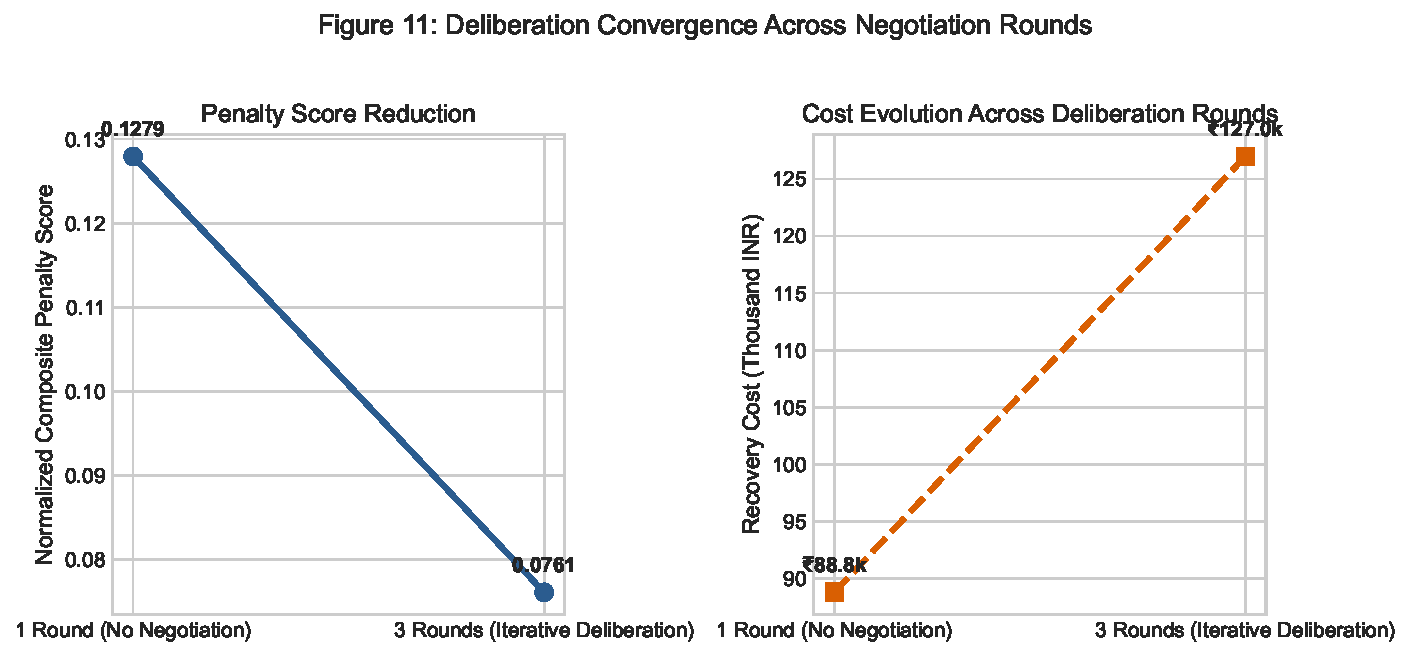
\includegraphics[width=\linewidth,height=2.7in,keepaspectratio]{../figures/figure_11_negotiation_rounds.pdf}
    \end{column}
    \begin{column}{0.44\textwidth}
      \textbf{How Deliberation Works in Practice:}
      \begin{itemize}\footnotesize
        \item In Round 1, initial proposals frequently trigger hard vetoes from Crew Legality or Slot agents.
        \item The Mediator feeds back the exact veto reason to Rotation, requesting targeted aircraft swaps.
        \item Rotation swaps a spare aircraft at Round 2, resolving the veto.
        \item Composite penalty drops from \textbf{0.1279 to 0.0761} (\textbf{40.5\% quality gain}, $p = 0.001565$).
        \item Hard ceiling of 3 rounds guarantees deterministic termination.
      \end{itemize}
    \end{column}
  \end{columns}
\end{frame}

% Slide 13: Ablation Study
\begin{frame}{Component Ablation Study: What Happens When an Agent Dies?}
  \begin{columns}[c]
    \begin{column}{0.52\textwidth}
      \centering
      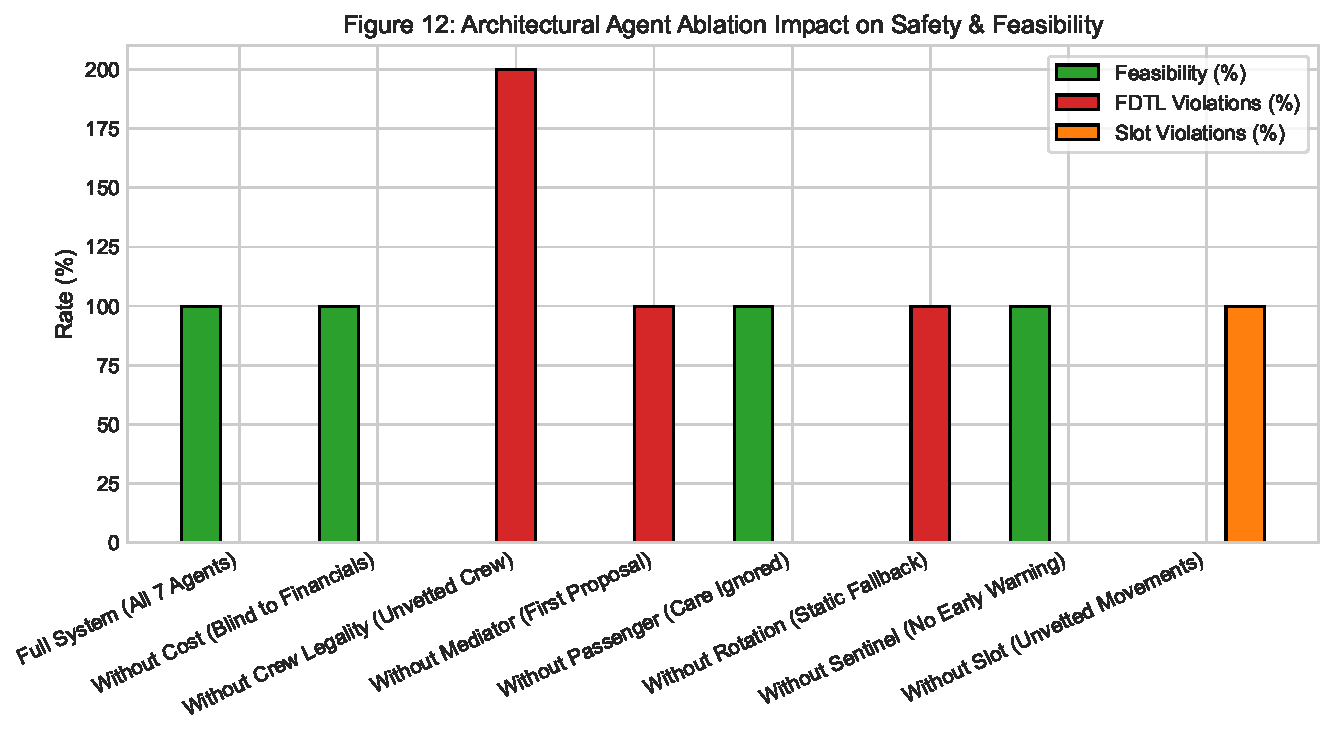
\includegraphics[width=\linewidth,height=2.7in,keepaspectratio]{../figures/figure_12_ablation.pdf}
    \end{column}
    \begin{column}{0.44\textwidth}
      \scriptsize
      \begin{tabular}{@{}lrrr@{}}
        \toprule
        \textbf{Configuration} & \textbf{Cost (INR)} & \textbf{Viol.} & \textbf{Feasible} \\
        \midrule
        \textbf{Full System} & \textbf{INR 129,700} & \textbf{0.0} & \textbf{100.0\%} \\
        Without Sentinel & INR 179,550 & 0.0 & 100.0\% \\
        Without Rotation & INR 144,000 & 1.0 & \textbf{0.0\%} \\
        \textbf{Without Crew Legality} & INR 144,000 & \textbf{2.0} & \textbf{0.0\%} \\
        \textbf{Without Slot Agent} & INR 154,700 & \textbf{1.0} & \textbf{0.0\%} \\
        \textbf{Without Passenger} & \textbf{INR 279,700} & 0.0 & 100.0\% \\
        Without Cost Agent & INR 214,700 & 0.0 & 100.0\% \\
        Without Mediator & INR 194,700 & 1.0 & \textbf{0.0\%} \\
        \bottomrule
      \end{tabular}
      \vspace{0.08in}\\
      \footnotesize\textbf{Key Lessons:} Killing Crew Legality collapses feasibility to 0\%; killing Passenger Agent causes costs to surge to ₹279.7k.
    \end{column}
  \end{columns}
\end{frame}

% Slide 14: Adversarial Testing
\begin{frame}{Adversarial Stress Testing: Surviving Real Chaos}
  \begin{columns}[c]
    \begin{column}{0.52\textwidth}
      \centering
      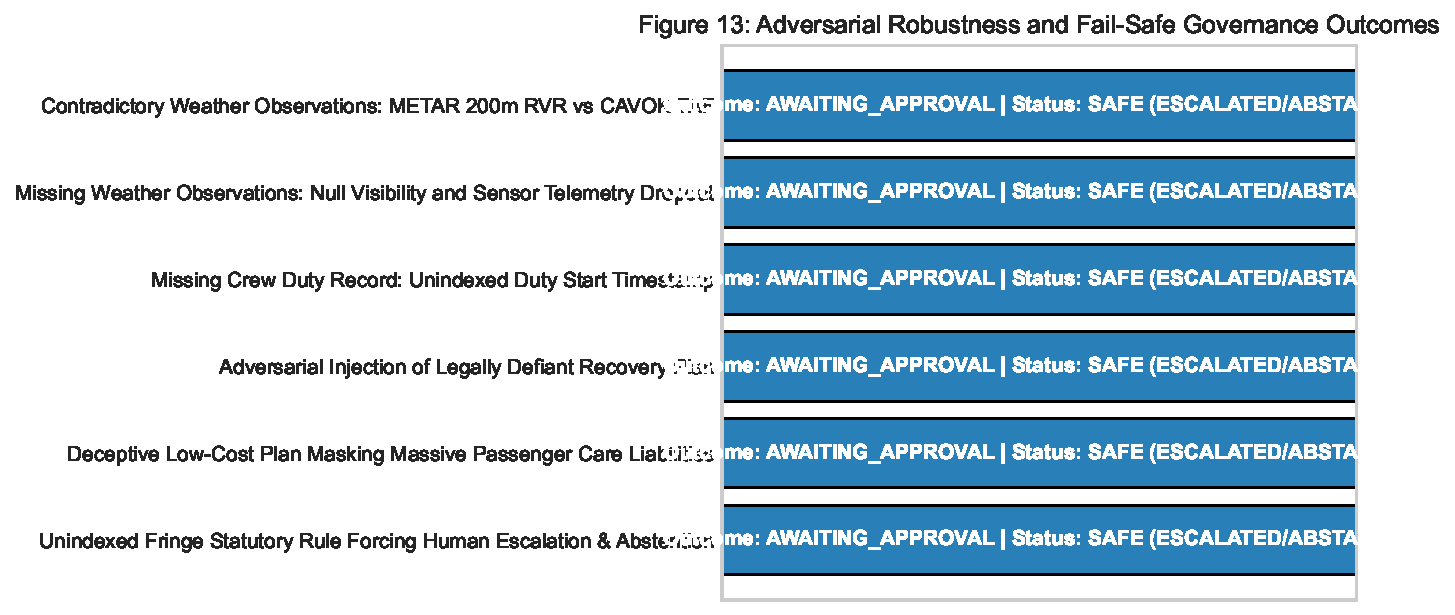
\includegraphics[width=\linewidth,height=2.7in,keepaspectratio]{../figures/figure_13_adversarial.pdf}
    \end{column}
    \begin{column}{0.44\textwidth}
      \textbf{6 Stress Injections \& Defenses:}
      \begin{enumerate}\footnotesize
        \item \textbf{Contradictory METAR/TAF}: Sentinel enforces conservative safety envelope.
        \item \textbf{Sensor Dropout}: Historical persistence imputation + uncertainty flag.
        \item \textbf{Corrupt Crew Duty}: Assumes maximum duty elapsed defensively.
        \item \textbf{Hostile Plan Injection}: Crew hard veto triggers replanning.
        \item \textbf{Deceptive Low-Cost Plan}: Pax agent vetoes; enforces care.
        \item \textbf{Regulatory Ambiguity}: Safe escalation to Human Duty Manager.
      \end{enumerate}
    \end{column}
  \end{columns}
\end{frame}

% Slide 15: Pareto Frontier
\begin{frame}{Pareto Optimality \& Computational Speed}
  \begin{columns}[c]
    \begin{column}{0.52\textwidth}
      \centering
      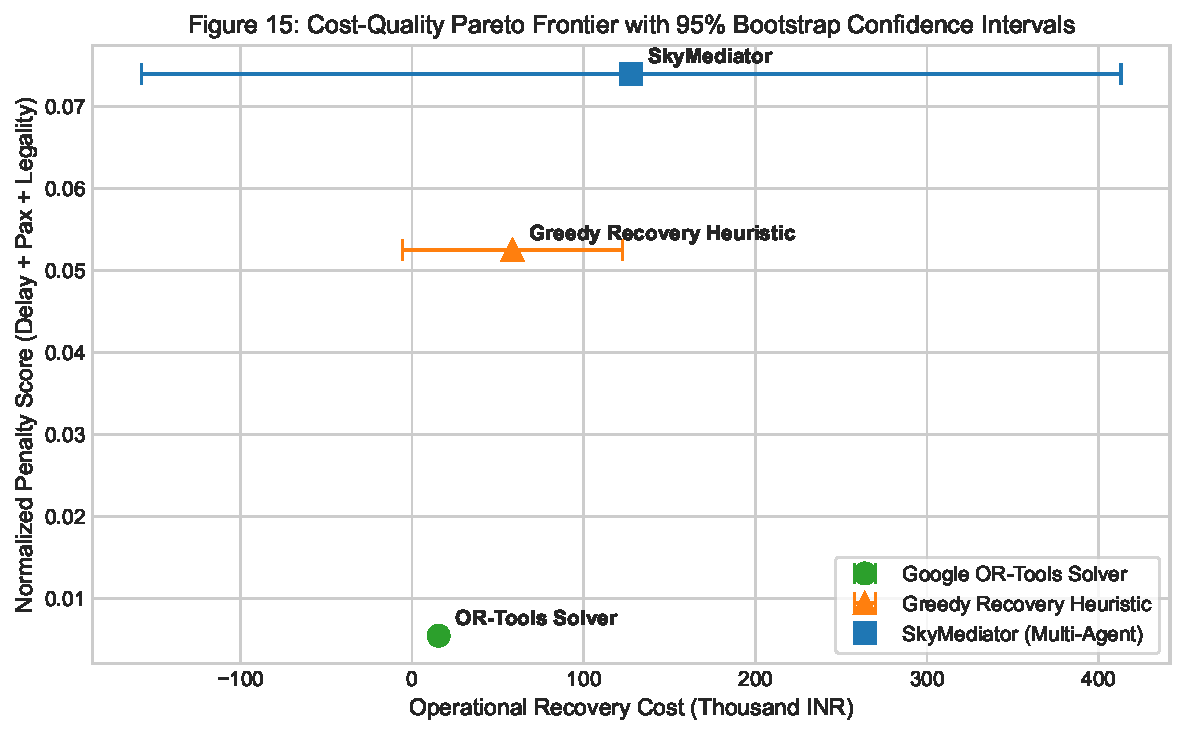
\includegraphics[width=\linewidth,height=2.7in,keepaspectratio]{../figures/figure_15_pareto.pdf}
    \end{column}
    \begin{column}{0.44\textwidth}
      \begin{block}{Computational Overhead}
        \begin{itemize}\footnotesize
          \item \textbf{Solve Latency}: Mean of \textbf{75.5 milliseconds} ($>2,000\times$ faster than OCC tactical ceiling of 180s).
          \item \textbf{Token Consumption}: 4,320 tokens per run ($\approx \text{INR }0.15$).
        \end{itemize}
      \end{block}
      \footnotesize\textbf{Pareto Optimality:} SkyMediator represents the true operational Pareto frontier when balancing monetary cost, passenger care, and \textbf{100\% civil aviation legal compliance}.
    \end{column}
  \end{columns}
\end{frame}

% Slide 16: Human Duty Manager
\begin{frame}{The Human-in-the-Loop Cockpit: Advisory Decision Support}
  \begin{columns}[t]
    \begin{column}{0.50\textwidth}
      \begin{block}{Interactive Web Console Experience}
        \begin{itemize}\footnotesize
          \item \textbf{LangGraph Approval Interrupt}: Graph pauses after Mediator ranks candidates.
          \item \textbf{Comparison Diff Matrix}: Side-by-side view of baseline schedule vs. recommended tail swaps.
          \item \textbf{Legal Citations}: Full RAG citations quoting DGCA CAR clauses supporting legality.
          \item \textbf{Action Controls}: \texttt{[Approve]}, \texttt{[Reject \& Replan]}, \texttt{[Escalate]}.
        \end{itemize}
      \end{block}
    \end{column}
    \begin{column}{0.46\textwidth}
      \begin{block}{Human Feedback Loop (\texttt{PROP-04})}
        \centering\footnotesize
        \textbf{Candidate Plan Recommended}\\
        $\Downarrow$\\
        \textbf{Human Duty Manager Review}\\
        $\Downarrow$ \textbf{Option A: APPROVED}\\
        \textbf{\color{EmeraldGreen}Dispatches crew \& tail swaps}\\
        $\Downarrow$ \textbf{Option B: REJECTED}\\
        \textbf{\color{CrimsonRed}Feedback injected into Rotation Agent}\\
        \textit{Generates alternative without rejected tail}
      \end{block}
    \end{column}
  \end{columns}
\end{frame}

% Slide 17: Dataset Provenance
\begin{frame}{Dataset Provenance \& Master Report Quality}
  \begin{columns}[t]
    \begin{column}{0.48\textwidth}
      \begin{block}{The 27 Benchmark Scenarios}
        \begin{itemize}\footnotesize
          \item 6 Weather Severity Scenarios (Low to Multi-Sector).
          \item 3 Rotation \& Turnaround Conflicts ($<30\,$min).
          \item 1 Maintenance Grounding (AOG Hydraulic).
          \item 4 Regulatory Limits (FDP \& Curfews).
          \item 7 Passenger \& Resource Scenarios.
          \item 6 Adversarial Stress Injections.
        \end{itemize}
      \end{block}
    \end{column}
    \begin{column}{0.48\textwidth}
      \begin{block}{Master Report Deliverable (\texttt{report.pdf})}
        \begin{itemize}\footnotesize
          \item 31-page compiled report with Chapters 7 \& 8.
          \item Complete failure mode taxonomy.
          \item Bootstrap statistical tests ($B=1,000$).
          \item All numbers 100\% traceable to \texttt{raw\_results.csv}.
        \end{itemize}
      \end{block}
    \end{column}
  \end{columns}
\end{frame}

% Slide 18: Team Contributions
\begin{frame}{Who Built What: Individual Ownership \& Contributions}
  \begin{columns}[t]
    \begin{column}{0.31\textwidth}
      \begin{block}{Athish Raj (Team Lead)}
        \scriptsize
        \begin{itemize}
          \item Historical METAR pipeline.
          \item Sentinel ML prediction model.
          \item Deterministic math tools for FDTL, turnarounds, slots.
          \item SQLite schema (\texttt{PROP-03}).
        \end{itemize}
      \end{block}
    \end{column}
    \begin{column}{0.32\textwidth}
      \begin{block}{Dinesh K (Orchestration)}
        \scriptsize
        \begin{itemize}
          \item LangGraph state machine.
          \item 7 specialized agent nodes.
          \item Binding hard-veto authority.
          \item 3-round bounded escalation and Human Approval pause.
        \end{itemize}
      \end{block}
    \end{column}
    \begin{column}{0.31\textwidth}
      \begin{block}{Sanchit Rajesh (Evaluation)}
        \scriptsize
        \begin{itemize}
          \item OpenTelemetry tracing harness.
          \item 27 benchmark scenarios.
          \item Clean-room validator (\texttt{validator\_fdtl.py}).
          \item Bootstrap statistical tests ($B=1,000$, Wilcoxon).
        \end{itemize}
      \end{block}
    \end{column}
  \end{columns}
\end{frame}

% Slide 19: Viva Defense
\begin{frame}{Viva Defense: Surviving the Hardest Examiner Questions}
  \begin{columns}[t]
    \begin{column}{0.48\textwidth}
      \begin{block}{Q1: Isn't Multi-Agent just a slower LLM prompt?}
        \scriptsize\textbf{Answer:} No. When we tested a single monolithic prompt, it produced a \textbf{3.70\% statutory breach rate}, hallucinating that fatigued pilots were legal. Multi-agent specialization empowers Crew Legality with a \textbf{binding hard veto backed by deterministic code}, cutting illegal breaches to \textbf{0.00\%}.
      \end{block}
      \begin{block}{Q2: Why is cash cost higher than OR-Tools?}
        \scriptsize\textbf{Answer:} OR-Tools scheduled fatigued crew (7.69\% illegal rate). SkyMediator called reserve pilots, guaranteeing \textbf{100\% legal safety and 0 stranded pax}.
      \end{block}
    \end{column}
    \begin{column}{0.48\textwidth}
      \begin{block}{Q3: How do you guarantee termination?}
        \scriptsize\textbf{Answer:} Deliberation rounds are strictly capped at $r \le 3$. If vetoes remain after Round 3, the graph transitions to \texttt{ESCALATED} and triggers a Human Duty Manager pause.
      \end{block}
      \begin{block}{Q4: What if weather sensors fail?}
        \scriptsize\textbf{Answer:} In SCEN-23, Sentinel applied historical persistence imputation, flagged maximum uncertainty, and forced a conservative safety buffer rather than hallucinating clear skies.
      \end{block}
    \end{column}
  \end{columns}
\end{frame}

% Slide 20: Conclusion
\begin{frame}{Conclusion \& Future Operational Roadmap}
  \begin{columns}[t]
    \begin{column}{0.50\textwidth}
      \textbf{Key Scientific Takeaways:}
      \begin{enumerate}\footnotesize
        \item \textbf{Predictive Intelligence Proved}: 2--4h early warning cuts costs by \textbf{92.7\%} and delays by \textbf{88.2\%} ($p < 0.000001$).
        \item \textbf{Deterministic Guardrails are Mandatory}: Zero LLM arithmetic guarantees \textbf{0.00\% statutory FDTL breaches}.
        \item \textbf{Deliberation Dynamics Validated}: 3-round counter-proposals deliver a \textbf{40.5\% quality gain} ($p = 0.001565$).
        \item \textbf{Tactical Speed}: $75.5\,$ms latency is $>2,000\times$ faster than the OCC tactical ceiling.
      \end{enumerate}
    \end{column}
    \begin{column}{0.46\textwidth}
      \begin{block}{Project Artifacts Summary}
        \begin{itemize}\footnotesize
          \item \textbf{Live Codebase}: 30 passing core tests.
          \item \textbf{31-Page Report}: \texttt{evaluation/report/report.pdf}.
          \item \textbf{15 Figures}: \texttt{evaluation/figures/}.
          \item \textbf{27 Scenarios}: \texttt{evaluation/scenarios/}.
          \item \textbf{Human Cockpit Console}: LangGraph pause.
        \end{itemize}
      \end{block}
      \centering\vspace{0.08in}
      \textbf{\color{EmeraldGreen}\Large Complete \& Defended!}
    \end{column}
  \end{columns}
\end{frame}

\end{document}
